\chapter{Physics, Mathematics and GR}\label{chap17}

\Authorline{B S Kiranagi\footnote{Adjunct Professor, Mangalore University, Mangalagangotri. (Dedicated to the affectionate memory of G, Ramachandran)}\footnote[*]{Email: \url{bskiranagi@yahoo.com}}}
\addtocontents{toc}{\protect\contentsline{section}{{\sl B S Kiranagi}\smallskip}{}}

\authinfo{Retired Professor, Department of Mathematics\\ University of Mysore}

I feel greatly honoured in being given this opportunity of paying a tribute of my reverence to the memory of my respected friend Gowrava\-ram Ramachandran (GR) who was a simple, sincere, hardworking honest man with tremendous knowledge of physics and philosophy, in particular Bhagavad Gita.

First I would like to quote from “Legacy of Learning” \cite{chap17-key01BSK}. It is a saga of higher education, wherein Mysore University is a hero, focusing not only on the happenings but also on strange silences, with an eye on tomorrow's prosperity. An eminent physicist Shashidhara Prasad writes in Achievements of DOS in Physics \cite{chap17-key02BSK}: “Prof.\ Ramachandran and his former student Dr.\ Mallesh who is presently working as a faculty are carrying out research work in theoretical nuclear physics, particle physics and spin physics for the last 25 years. Some of the work was done in collaboration with the premier institutions of the country like TIFR, Matscience, ISRO, CTS at IISC. and Aligarh Muslim University. Mathematical techniques developed by this group have been used to discuss such diverse phenomena as Einstein-Podolosky-Rosen-Bohm paradox, Observables in Radar Polarimetry, Pancharathnam Geometric formula etc.... ”

I had the great privilege of joining the services in the Department of Mathematics, Mysore University, as Associate Professor in 1982. I had often participated in lectures given by famous physicists in IMSc, Madras University, University of Hyderabad and Mysore University. I had many discussions with Professor GR to understand things, in particular, to understand the applications of Lie groups to physics as my topic of research is “Lie algebra and Lie group bundles”. Many times, I felt that I knew nothing in mathematics while discussing with Prof.\ GR. I fear very much that it may not be possible for me to write about him academically. But it gives me great pleasure indeed to be invited to write a few words about my academic relationship and casual chats which turned into discussions on physics, philosophy, mathematics and concerned scientists, mathematicians, philosophers. Most of the time we chatted across the common compound wall of our Gangotri quarters during the years 1992 to 1998 as I was blessed to be his neighbour. Soon we became family friends. Sometimes I heard him chanting mantras while performing poojas. During Krishna Janmashtami and during Karthika they used to put a lot of oil lamps all over the compound walls, but he was not orthodox personally. He knew the philosophy of all religions and had equal respect for them. For him everyone is a part of Godliness and he respected everyone equally. Literally he believed in hard work as he used to feel that the society had given so much to him, that he owed very much to the society. He thought he could pay back to society by being simple, sincere, honest to all and by being a dedicated researcher in physics. He never used to talk about anything other than mathematical sciences and about scientists. For him meditation, chanting religious slokas, listening to religious music, poojas, reading philosophy and the Hindu newspaper were perhaps his activities for relaxation.

\textbf{I will now present some of our casual talks on Mathematical sciences, Physics and Religion.}

These discussions influenced me to have a personal copy of the book \cite{chap17-key04MJL}.  

\textbf{BSK:} Has a strong belief in the teachings of any particular religion influenced any person to come out with good research in physics?

\textbf{GR:} Yes, Murray Gell- Mann (1929 to 2019), a believer of Buddhism and his saying  ``Now this, O monks, is the noble truth of the way that leads to the cessation of pain: this is the noble Eightfold Way, namely, right views, right intention, right speech, right action, right living, right effort, right mindfulness, right concentration”. He devised a scheme to codify particles, grouping all those known into eight families — the “Eightfold Way”. In 1961, Gell-Mann and, independently, Yuval Ne’eman, employed the special Unitary group SU(3) to unify strangeness with nuclear isospin. It led to the classification of particles by SU(3) multiplets, which Gell-Mann called the Eightfold Way, the noble Eightfold path of Buddhism. That was pioneering work in the use of Lie Group theory to understand particle physics. He said there are many particles like mesons etc. His contributions include many   fundamental ideas, such as the renormalisation group, which is fundamental to quantum field theory and statistical mechanics.  He received the 1969 Nobel Prize for “his contributions and discoveries concerning the classification of elementary particles and their interactions”. In the early 1950s, he proposed a new quantum number, called strangeness, to explain the unusual properties of novel strongly interacting particles seen in cosmic rays. Strangeness proved to be a successful organising principle of the vast spectrum of particles that subsequently emerged in accelerator experiments.

\section*{Physics and Patriotism\\ {\large Homi Bhabha and Harish-Chandra}}

At my humble request GR wrote an article \cite{chap17-key03GR} “On Harish-Chandra's contributions to particle physics”. Soon it will appear in my book “On Harish-Chandra” which I have informed him just before his passing away.

\textbf{BSK:} Whom do you respect in India among theoretical physicists and why?

\textbf{GR:} To mention a few, I respect Nobel Laureate C V Raman (1888--1970) who made groundbreaking work in the field of \underline{light scattering}. He discovered that when light traverses a transparent material, some of the deflected light changes wavelength and amplitude. This phenomenon was a new type of scattering of light and was subsequently known as the Raman effect (\underline{Raman scattering}). Raman was the first Asian to receive a Nobel Prize in any branch of science.

And Satyendra Nath Bose (1894--1974), FRS, known for\break Bose-Einstein statistics and the theory of the Bose-Einstein condensate. The class of particles that obey Bose-Einstein statistics, \underline{bosons}, was named after Bose by \underline{Paul Dirac}.

An ideal \textbf{Bose gas} is a quantum-mechanical \underline{phase of matter}, analogous to a classical \underline{ideal gas}. It is composed of \underline{bosons}, which have an integer value for spin, and obey \underline{Bose-Einstein statistics}. The statistical mechanics of bosons were developed by \underline{Satyendra Nath Bose} for a \underline{photon gas}, and extended to massive particles by \underline{Albert Einstein} who realized that an ideal gas of bosons would form a condensate at a low enough temperature, unlike a classical ideal gas. This condensate is known as a \textbf{\underline{Bose-Einstein} condensate}.

\textbf{BSK: Who is mainly responsible for the development of science and mathematics in India.}

\textbf{GR:}  A great visionary, Homi Jehangir Bhabha (30-10-1909 to 24-1-1966), is responsible for our research in atomic energy and the advance that we have made in that science. He excelled in mathematical studies under Nobel Laureate Paul Dirac during his mathematics degree course.  He completed his doctoral studies in theoretical physics under \underline{Ralph H. Fowler}. During his research fellowship, he split his time working at Cambridge and with Nobel Laureate \underline{Niels Bohr} in Copenhagen. Bhabha published a paper in the \textit{Proceedings of the Royal Society, Series A}, in which he presented the first calculation to determine the cross section of electron-positron scattering. Electron-positron scattering was later named \underline{Bhabha scattering}, in honour of his contributions to the field. For him, the nation came first.
\vskip 1pt

\textbf{BSK:} Who is responsible for the development of Atomic Energy and Space research in India.
\vskip 1pt

\textbf{GR:} Bhabha established the Atomic Energy Commission, serving as its first Chairman, and developed Atomic Energy for peaceful purposes. After his death, the Atomic Energy establishment in Mumbai was renamed as the Bhabha Atomic Research Centre in his honour. Bhabha is known as the Father of the Indian nuclear energy programme. He later served as the member of the \underline{Indian Cabinet}'s Scientific Advisory Committee and provided the pivotal role to Vikram Sarabhai to set up the Indian National Committee for Space Research.
\vskip 1pt

\textbf{BSK:} Sir, do you know the great mathematician Harish-Chandra who joined Bhabha on the advice of Krishnan and C. V. Raman. Harish-Chandra spent two years (1943--1945) in IISc with eminent physicist Homi J. Bhabha before proceeding to work with Nobel Laureate Dirac with Bhabha’s recommendations.  Bhabha had a great vision of science and he had initiated the creation of Tata Institute of Fundamental Research in Bombay by using his cordial relationship with the great philanthropist J. R. D. Tata.  The Tata Institute of Fundamental Research is a monument to his knowledge of architecture, and his understanding of how to combine functional needs with aesthetic perfection. Academically it is worth visiting. It is located in Colaba in the west of Mumbai on the seashore with serene natural beauty. It is one of the best research institutes of Mathematics in the world.

I just quote a proposal \cite{chap17-key09SM} of Bhabha in 1944 to Sir Dorab J Tata for establishing a vigorous school of research in fundamental physics and mathematics.  He wrote:  ``......... It is absolutely in the interest of India to have a vigorous school of research in fundamental physics, for such a school forms the spearhead of research not only in less advanced branches of physics but also in problems of immediate practical application in industry. \textbf{If much of the applied research done in India today is disappointing or of very inferior quality it is entirely due to the absence of sufficient number of outstanding pure research workers who would set the standard of good research and act on the directing boards in an advisory capacity ...} Moreover, when nuclear energy has been successfully applied for power production in say a couple of decades from now, India will not have to look abroad for its experts but will find them ready at hand……".

\textbf{GR:} Can you enlighten me briefly about Harish-Chandra and his work broadly? 

\textbf{BSK: I quote everything from [BSK]} To every Indian Harishchandra means Satya Harishchandra, the king of Kosala region, which is on the banks of river Sarayu of ancient India, who was known for his extraordinary truthfulness and duty. Bearing the name of this illustrious king, the mathematician \textbf{Harish Chandra (1923-1983)} is known for his groundbreaking work on Lie theory. Harish Chandra goes down in the history of mathematics as the greatest Indian mathematician after the legendary Srinivasa Ramanujan (1887-1920). Harish Chandra and Ramanujan were easily the two greatest Indian mathematicians of the last century. While the latter is a household name in India, Harish Chandra, despite his sustained and seminal contributions to representation theory of semisimple Lie Groups, remains relatively unknown. His work is too technical. Harish started his research career as a physicist under Nobel laureate P.A.M.Dirac in Cambridge University before moving on to a very successful career as a mathematician at the Institute for Advanced Studies in Princeton.

\textbf{GR:} Then what made him switch over to mathematics. Though he had obtained his Ph.D under the supervision of Dirac and his work appeared in physics books.

\textbf{BSK: Physics to Mathematics:}  Harish had dreamt of devoting his life to theoretical physics after seeing the book of Dirac on Principles of Quantum Mechanics in the Allahabad University Library in 1940. However slowly a new hunger grew in him- the desire to take up research in Lie Groups. He learned mathematics to some extent from studying great books, but mainly by rediscovering truths by himself. That was the power of expressing his strong intuition into mathematical proof. Harish chose the long and difficult road to mathematics. During the time with Dirac, partly as a student in Cambridge and partly in the Institute for Advanced Studies, Princeton, New Jersey, which Dirac visited in 1947-48 taking him along as his assistant, Harish-Chandra abandoned physics and turned to mathematics. He was eager to conquer all that was best or most exciting at that time, and started taking courses on Lie algebras and class field theory from Chevalley and Emil Artin at Princeton, and then moving on to Harvard to study algebraic geometry with Zarisky. In Cambridge he attended the lectures by J.E. Littlewood and Philip Hall and started discovering mathematics and he began to doubt his career as a physicist. Harish commented that: “Soon after coming to Princeton, I became aware that my work on the Lorentz Group was based on somewhat shaky arguments.  I had naively manipulated unbounded operators without paying any attention to their domains of definition. I once complained to Dirac about the fact that my proofs were not rigorous and he replied “I am not interested in proofs but only in what nature does”.  This remark confirmed my growing conviction that I did not have the mysterious sixth sense which one needs in order to succeed in physics and I soon decided to move over to mathematics”. One can thus see the evolution in Harish Chandra’s career - Krishnan, Homi Bhabha, Dirac, Chevalley and his ideas on relativistic field theory which found its way into some famous texts.

\textbf{GR:} Perhaps the comment of Dirac, and his innate love for mathematics, changed him, though Harish and Dirac were bound by the affinity between souls.

\textbf{BSK:} Yes, that is true.  Abel Laureate Robert Langlands has the following to say about the greatness of Harish in mathematics \cite{chap17-key07RPL} : “Harish-Chandra was one of the outstanding Mathematicians of his generation, an algebraist and analyst, and one of those responsible for transforming infinite dimensional Group representation theory, from a modest topic on the periphery of mathematics and physics, into a major field central to contemporary mathematics”. The unique greatness of Harish can be summed up in the words of one of the best mathematicians of $20^{\rm th}$ century, Armand Borel (1923-2003) [AB], “Later I heard several times André Weil say that he knew only two mathematicians for whom technical difficulties simply did not exist, namely Chevalley and Harish Chandra.  However, this was technical power at the service of the highest goals. \textbf{I would be hard put to give another example of a work by a single author extending over 2000 pages at such a consistently high level, or should I say relentlessly high level, devoted to one main goal, very broadly conceived.”}  The main goal of determination of the general Plancherel formula for semisimple Lie Groups was achieved by Harish Chandra in 1976, which is his magnum opus on representation theory, called “Harmonic Analysis on Semisimple Lie Groups” 

\textbf{GR:} Any other interesting and noted facts about Harish-Chandra?

\textbf{BSK:}  I will just quote three facts.

1).~Once Dirac took Harish-Chandra as his assistant to  the Institute for Advanced Study (IAS). After attending  lectures in mathematics by an eminent mathematician,  it seems Harish-Chandra asked that mathematician how do I know that I am good at mathematics? You take any standard book or a research paper by a well known mathematician in your field of interest and read only definitions and try to prove theorems by yourself. If you are able to prove it by yourself or if you are able to give alternative proofs, think that you are going to be one of the best mathematicians in the world. There he decided to take up mathematics.

IAS, located in Princeton, New Jersey, in the United States, is an independent postdoctoral research center for theoretical research and intellectual inquiry. It is perhaps best known as the academic home of Albert Einstein, J. Robert Oppenheimer, Hermann Weyl, John von Neumann and Kurt Gödel, after their immigration to USA. {\small Later it became the academic home of Harish-Chandra.}

2). The Harish-Chandra Research Institute (HRI) is a premier institution dedicated to research in Mathematics and Theoretical Physics , located in Allahabad (officially Prayagraj), Uttar Pradesh in \underline{India}. Mehta  Research Institute was renamed in honor of renowned Indian mathematician, \underline{Harish-Chandra} in 2000.

\textbf{3) Seminars on Harish-Chandra’s work}

In seminars on Harish-Chandra’s work in  Institut des Hautes Études Scientifiques(IHES), France, one of the best institutes in the world, there were many eminent mathematicians like J. P. Serre, Deligne, Tits, Cartier and many others.  Often a discussion would start among this elite group with a quest like why is it that Harish-Chandra has built up such a wide base to prove this particular result?  He would have solved it by using such and such techniques. Once I heard somebody remarking that: “Yes, I see what you mean. I have given the simple proof for this particular result and taken away the beauty of the techniques.” Oh perhaps this technique will help to solve further results or it is the same technique which can be used to solve all other similar results in other branches.  There they used to name many theorems as Harish-Chandra’s theorems, Harish-Chandra’s modules….  \textbf{Once eminent mathematician and physicist V S Varadarajan of the USA told me that “there are two ways to become famous in mathematics; one is V.K. Patodi’s way and the other is Harish-Chandra’s”.} Vijay Kumar Patodi (1945--1976) became famous overnight by deriving the Atiyah-Singer index theorem by another approach using Heat kernel functions. And for an analytic proof of the Riemann-Roch-Hirzebruch theorem for Kähler manifolds which extended the methods of his earlier paper “curvature and the eigen forms of the Laplace operator” to a much more complicated situation.
\vskip 2pt

\textbf{GR:} Is there any central theme of mathematics to which both Harish Chandra and Ramanujan have made significant contributions?
\vskip 2pt

\textbf{BSK:} Here we present an introduction to a central theme of mathematics to which both Ramanujan and Harish Chandra have made significant contributions. For mathematical details refer to the excellent article by the eminent mathematician V. Kumar Murty \cite{chap17-key10VKM}. Ramanujan had a powerful mathematical imagination.  Everyone has great sympathy for the severe conditions under which Ramanujan worked and have great admiration for his achievements and gifts. There can be no doubt that Ramanujan was a genius. His death at such an early age was a really tragic event for the development of mathematics.
\vskip 2pt
 
The eminent mathematician G.H.Hardy, who was responsible for Srinivasa Ramanujan (1887-1920) becoming known internationally,\break writes about Ramanujan as follows: “The limitations of his knowledge were startling as its profundity. Here was a man who could work out modular equations and theorems of complex   multiplication to orders unheard of..., who had discovered by himself the functional equation of the Zeta function, but had never heard of a doubly periodic function or Cauchy’s theorem,  and had indeed the vaguest idea of what a function of a complete variable was”.
\vskip 2pt
 
Similarly Abel Laureate Langlands \cite{chap17-key06RPL} writes of Harish Chandra that “he came to mathematics relatively late and, in spite of enthusiastic initial attempts, there were broad domains of mathematics that he never assimilated in any serious way, although he learned all that he needed... it is not too much of an exaggeration to say that he manufactured his own tools as the need arose, and that one of the grand mathematical theories of this century has been constructed with the skills with which one completes a course in advanced calculus.
\vskip 2pt
 
Ramanujan did not go through the usual educational process,\break whereas Harish-Chandra was well trained in the usual educational process.  It is certainly of great interest and importance to figure out the eminent mathematician’s thinking process and to try to understand the architecture of their everlasting achievements. Analyzing clearly and thinking deeply about the research problems along with the deep desire to solve them perhaps makes men to visualize the architecture of the solutions to the research problems. So, it is necessary to create the atmosphere of deep love first for the subject.  I quote V. Kumar Murthy about Ramanujan and Harish Chandra: “In the infinite ocean of time, even great thinkers must seem like floating wisps of straw. But through our human perspective, we see them as great flagships and spacious ferries, and draw inspiration from their life and work. Mathematical contributions aside, it is clear that both Ramanujan and Harish Chandra have inspired many mathematicians all around the world and will continue to do so in the decades to come”
 
\section*{M. F. Atiyah and Donaldson, 1986.}

GR got me bulky research papers of Donaldson and Freedman, perhaps through his student M. V. N. Murthy.
  
\textbf{BSK:} Sir, often I refer to the book on K-theory by M. F. Atiyah, whom I have met  and have attended his lectures at TIFR, Mumbai. He was awarded the Fields Medal and Abel Prize for his discovery and proof of the index theorems. His outstanding role, along with others, in building new bridges between mathematics and theoretical physics is well known. Mathematical models are almost always described by a system of differential equations. To make use of the model one seeks the solutions to this system of differential equations, but these can be almost impossible to find. The critical new insight of Atiyah and Singer was that it is much easier to answer a slightly different question, namely: “How many solutions are there?” The Atiyah-Singer index theorem gives a good answer to this question. The point is that it is not necessary to find the solutions of the system to get to know how many solutions exist. Conversely, a knowledge of the number of solutions can in fact make it easier to find the solutions. Vijay Kumar Patodi is known for the Atiyah-Patodi-Singer index [NHP14].

\textbf{BSK:} GR Sir, once I heard that Atiyah was watching, through his office window, a boy trying to climb a smooth wall which was almost impossible. He offered to take the boy as a research student and put him to work on the long-standing problem of solving other structures of Euclidean 4-space ${\rm R}^{4}$ and their relevance to physics.

\textbf{GR:} Interesting, who was that boy?

\textbf{BSK:} He was Sir Simon Kirwan Donaldson. In 1982, as a research student, he proved what is known as the diagonalizability theorem \cite{chap17-key08SD}, and went on to open up a whole new area in four-dimensional geometry. This stunned the mathematical world. Together with the important work of Michael Freedman, Donaldson's result implied that there are “exotic” 4-spaces, i.e., 4-dimensional differentiable manifolds which are topologically, but not differentiably, equivalent to the standard Euclidean 4-space  ${\rm R}^{4}$ .What makes this result so surprising is that n = 4 is the only value for which such exotic spaces exist. These exotic 4-spaces have the remarkable property that (unlike ${\rm R}^{4}$) they contain compact sets which cannot be contained inside any differentiably embedded 3-sphere!
\vskip 1pt

\textbf{GR:} In other words, if n is not equal to 4, then any smooth manifold homeomorphic to ${\rm R}^{\rm n}$ is diffeomorphic to ${\rm R}^{\rm n}$.
\vskip 1pt

\textbf{BSK:}  Yes, we experience the world in three dimensions: up and down, left and right, forward and backward. But according to Einstein, there are actually four: his theory of general relativity integrates time with the three spatial dimensions. While we cannot visualize four dimensions, we can analyze them mathematically. Donaldson has transformed our understanding of four-dimensional shapes, showing which ones can be “tamed” with the kind of equations that mathematicians can solve, and which cannot. In the process, he provided powerful new tools to physicists and also incorporated new ideas from physics into mathematics.
\vskip 1pt

\textbf{GR:} Can you highlight the speciality of Donaldson?
\vskip 1pt

\textbf{BSK:} Certainly. He proved results in pure mathematics by using physics. That is, Donaldson’s work is rather remarkable in its reversal of the usual direction of ideas from mathematics being applied to solve problems in physics. In particular he used the Yang-Mills equations, which are generalizations of Maxwell electromagnetic equations, to solve problems in pure mathematics.  His work has helped physicists to understand theories of space-time and how matter behaves at sub-nuclear levels much better. For his work, Donaldson used ideas and techniques from different fields due to which areas such as topology, physics, differential equations and geometry have become interwoven in ways that no one would have predicted half a century ago.

\section*{String theory and Sunil Mukhi in\\ Mysore - 1999, February.}

Professor GR gave me Sunil Mukhi’s lecture notes on Topology and Differential Geometry and told me that “Sunil Mukhi is an Indian theoretical physicist working in the areas of \underline{string theory, quantum field}\break \underline{theory} and \underline{particle physics}. He will be lecturing on mathematics which is necessary for theoretical physics in our Department. You may like his lectures on mathematics”.

\textbf{BSK:} What is string theory? Who are the experts in string theory till today in India?

\textbf{GR:} Till today (i.e.\ upto 1999), I know two physicists who work in string theory, one is Ashoke Sen, FRS, at Harish-Chandra Research Institute, Prayagraj (then called Allahabad) and the other is Sunil Mukhi at TIFR, Mumbai. String theory is a theoretical framework in Physics in which point-like particles are modeled as one dimensional objects called strings. Thus, string theory proposes that fundamental objects constituting the universe are one-dimensional strings. This theory is an overarching framework that can explain the physical reality. It tries to do so by suggesting that particles are actually one-dimensional string-like entities whose vibrations determine the particle’s properties, such as their mass and charge.

\textbf{BSK:} What is the advantage of considering particles as one-\break dimensional objects? Is there any advantage?

\textbf{GR:} Yes, there is some advantage. In 1984, Michael Green and John H Schwartz produced equations that showed how strings avoided certain inconsistencies plaguing other models that described particles as point-like objects. However, we have to wait and see whether this theory completely explains all of physics.

Whenever somebody got a Nobel Prize in Physics or a Fields Medal or Abel Prize in Mathematics, we would discuss their work.

\textbf{``We find all the more worthy of reverence the memory of those who tragically sacrificed their personal interest or comforts for\break achieving their higher and laudable noble objectives"}

\textbf{``There is no better education policy than having good teachers"}

\begin{thebibliography}{99}
\itemsep=0pt
\bibitem[BSK]{chap17-key01BSK} B. S. KIRANAGI, Legacy of Learning, Edited by V. G. Talawar and B. S. Kiranagi, published by University of Mysore.

\bibitem[BSK]{chap17-key02BSK} B. S. KIRANAGI, Harish-Chandra: A Mathematical Genius, Preprint of a Book 

\bibitem[GR]{chap17-key03GR} T Santhanam, G Ramachandran, G Padmanabhan, The relativistic covariance of wave equations for particles in Physics: Harish Chandra's contributions, Book ``On Harish Chandra”, Kiranagi B. S., Preprint of a Book

\bibitem[MJL]{chap17-key04MJL} Fundamentals of Elementary Particle Physics by Michael J.\ Longo.

\bibitem[NH]{chap17-key05NH} Nigel Hitchin, Sir Michael Atiyah OM, Biographical Memoirs of the Fellows of the Royal Society, 2020.

\bibitem[RPL]{chap17-key06RPL} R. P. Langlands, Harish Chandra, 1923--1983, Biographical Memoirs of the Fellows of the Royal Society, Vol.\ 31, pp.\ 197--225, 1985.

\bibitem[RPL]{chap17-key07RPL} R. P. Langlands, Recollections of the Harish Chandra and Reflections upon his career, Institute for Advanced Study, Princeton, U.S.A 1984.

\bibitem[SD]{chap17-key08SD} Donaldson, S. K., An application of gauge theory to four-dimensional topology, Journal of Differential Geometry, 18(2), 279--315, 1983.

\bibitem[SM]{chap17-key09SM} Dr Subodh Mahanti,  \underline{Homi Jehangir Bhabha Archived} 21 July 2011 at the \underline{Wayback Machine}. Vigyanprasar.gov.in. Retrieved on 30 June 2015.

\bibitem[VKM]{chap17-key10VKM} V Kumar Murthy, Ramanujan and Harish Chandra, The Mathematical Intelligencer, Vol.\ 15, No.\ 2, 1993, Springer-Verlag, New York.

\end{thebibliography}
\vskip 1cm

\centerline{\includegraphics[scale=.5]{authorsphotos/Prof_B_S_Kiranagi.eps}}
\bigskip

\noindent
\textbf{Dr.\ B. S. Kiranagi} obtained the Ph.D. degree in 1976 from Universite de Paris sud XIII, Orsay, France. He worked as a Lecturer in the Department of Mathematics, Madras University PG Center at Coimbatore, from 1978 to 1982. He joined the Department of Mathematics, Mysore University, as a Reader in 1982 and retired from there as Professor in 2003. He was NBHM Visiting Professor at the University of Hyderabad from May 2004 to May 2005. From 2009 to 2011 he was UGC Emeritus Professor at University of Mysore. He continued his research work at the University of Mysore from 2005 to 2018 through 3 research projects funded by DST. He was a neighbour of Prof.\ G. Ramachandran in the residential campus of Manasagangothri and they became close friends. Currently he is an Adjunct Professor at the Department of Mathematics, Mangalore University.
